\def\chapdir{./Chapter03}

\chapter{Requirements Analysis} \label{ch:requirements}

\section{Stakeholder Analysis}

\subsection{Identification of Key Stakeholders}

The OllamaNet platform serves a diverse group of stakeholders with varying needs and interests:

\begin{enumerate}
   \item \textbf{End Users}
   \begin{itemize}
      \item Regular users seeking full Context LLM powered conversations
      \item Knowledge workers and researchers
      \item Engineers and developers
      \item Students and educators
   \end{itemize}

   \item \textbf{Administrative Personnel}
   \begin{itemize}
      \item Platform administrators
      \item System operators
      \item Security administrators
      \item DevOps engineers
   \end{itemize}

   \item \textbf{Organization Stakeholders}
   \begin{itemize}
      \item IT departments
      \item Management teams
      \item Security and compliance teams
      \item Model development teams
   \end{itemize}

   \item \textbf{Technical Stakeholders}
   \begin{itemize}
      \item Frontend application developers
      \item Integration partners
      \item API consumers
      \item Infrastructure providers
   \end{itemize}

   \item \textbf{Governance Stakeholders}
   \begin{itemize}
      \item Data privacy officers
      \item Compliance managers
      \item Legal representatives
      \item Information security officers
   \end{itemize}
\end{enumerate}

\begin{figure}[p]
    \centering
    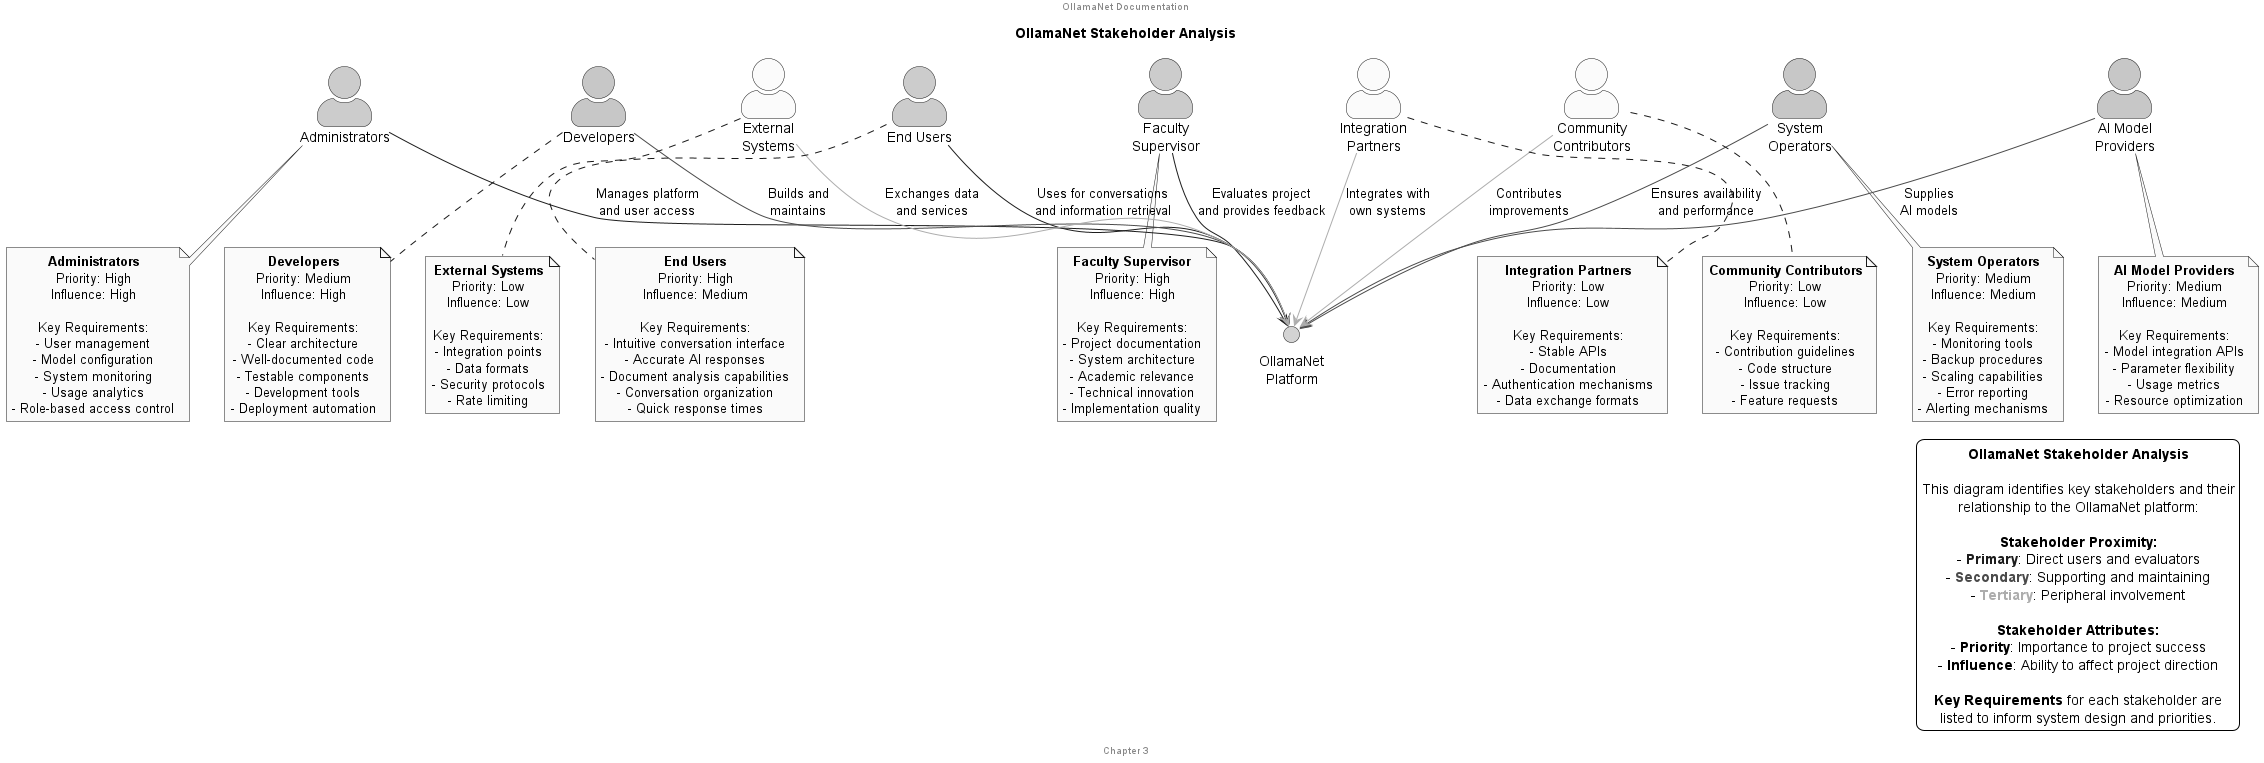
\includegraphics[width=\textwidth]{./Chapter03/figures/Stakeholder_Analysis.png}
    \caption{Stakeholder Analysis Diagram}
    \label{fig:stakeholder-analysis}
\end{figure}
\clearpage

\subsection{Stakeholder Needs and Concerns}

\subsubsection*{End User Needs}
\begin{itemize}
   \item Intuitive and responsive user interface
   \item Persistent conversation history
   \item Well-organized conversation management
   \item Fast and accurate AI responses
   \item Data privacy and security
   \item Seamless authentication
   \item Consistent experience across sessions
   \item Search capabilities for past interactions
   \item Access to a variety of AI models
\end{itemize}

\subsubsection*{Administrative Personnel Needs}
\begin{itemize}
   \item Comprehensive user management capabilities
   \item Fine-grained access control
   \item System monitoring and analytics
   \item Model deployment and management tools
   \item Platform configuration controls
   \item Efficient troubleshooting capabilities
   \item Audit and compliance features
   \item Task automation
\end{itemize}

\subsubsection*{Organization Stakeholders' Concerns}
\begin{itemize}
   \item Total cost of ownership
   \item Compliance with organizational policies
   \item Data security and privacy
   \item User productivity and efficiency
   \item Integration with existing systems
   \item Customization capabilities
   \item Governance and oversight
\end{itemize}

\subsubsection*{Technical Stakeholders' Needs}
\begin{itemize}
   \item Well-documented APIs
   \item Reliable service availability
   \item Consistent data models
   \item Proper error handling
   \item Scalable architecture
   \item Performance optimization
   \item Testability and debugging support
\end{itemize}

\subsubsection*{Governance Stakeholders' Concerns}
\begin{itemize}
   \item Regulatory compliance (GDPR, CCPA, etc.)
   \item Data residency requirements
   \item Audit trails and reporting
   \item Security controls and monitoring
   \item Risk management
   \item Intellectual property protection
\end{itemize}

\subsection{Priority Matrix of Stakeholder Requirements}

The following matrix presents the relative priority of key requirements across different stakeholder groups, rated as High (H), Medium (M), or Low (L) priority:

\begin{table}[h]
  \centering
  \caption{Priority Matrix of Stakeholder Requirements}
  \label{tab:requirement-priority}
  \begin{tabular}{|l|c|c|c|c|c|}
    \hline
    \textbf{Requirement} & \textbf{End Users} & \textbf{Admins} & \textbf{Organization} & \textbf{Technical} & \textbf{Governance} \\
    \hline
    Conversation Persistence & H & L & M & L & M \\
    \hline
    Model Discovery & H & M & M & L & L \\
    \hline
    User Authentication & M & H & H & M & H \\
    \hline
    Admin Controls & L & H & H & L & M \\
    \hline
    Performance & H & M & M & H & L \\
    \hline
    Security & M & H & H & M & H \\
    \hline
    API Access & L & M & L & H & L \\
    \hline
    Data Management & M & H & M & M & H \\
    \hline
    Scalability & L & H & H & H & L \\
    \hline
    Compliance & L & M & H & L & H \\
    \hline
  \end{tabular}
\end{table}

\subsection{Conflicting Requirements and Resolution Approach}

Several areas of potential conflict have been identified between different stakeholders' requirements:

\begin{enumerate}
   \item \textbf{Performance vs. Security}
   \begin{itemize}
      \item \textbf{Conflict}: End users prioritize fast response times, while security stakeholders require thorough validation and protection measures that may introduce latency.
      \item \textbf{Resolution}: Implement performance-optimized security measures, such as caching JWT validation results, using distributed authentication, and implementing parallel processing where possible.
   \end{itemize}

   \item \textbf{Usability vs. Compliance}
   \begin{itemize}
      \item \textbf{Conflict}: Seamless user experience may conflict with compliance requirements for explicit consents and disclosures.
      \item \textbf{Resolution}: Design user-friendly compliance features that integrate organically into the workflow, such as progressive disclosure of terms and just-in-time consent mechanisms.
   \end{itemize}

   \item \textbf{Flexibility vs. Governance}
   \begin{itemize}
      \item \textbf{Conflict}: Technical stakeholders want maximum flexibility and customization, while governance stakeholders require standardization and controlled processes.
      \item \textbf{Resolution}: Implement a modular architecture with clear extension points, coupled with governance policies on which aspects can be customized and how changes are managed.
   \end{itemize}

   \item \textbf{Notebook-First Architecture vs. Reliability}
   \begin{itemize}
      \item \textbf{Conflict}: The InferenceService's notebook-first architecture provides flexibility but creates challenges for reliability and management.
      \item \textbf{Resolution}: Implement robust service discovery mechanisms, monitoring, and auto-recovery while preserving the flexibility of the notebook environment.
   \end{itemize}

   \item \textbf{Centralized vs. Distributed Data}
   \begin{itemize}
      \item \textbf{Conflict}: Performance and user experience benefit from distributed caching, while governance and management prefer centralized control.
      \item \textbf{Resolution}: Implement a hybrid approach with a primary centralized database of record and distributed caching with clear invalidation strategies.
   \end{itemize}
\end{enumerate}

\begin{terminology}
\begin{description}
    \item[Stakeholder:] Any person, group, or organization with an interest in or concern about the project
    \item[Requirements Priority Matrix:] A visualization showing the relative importance of requirements to different stakeholders
\end{description}
\end{terminology}

\section{Functional Requirements}

\subsection{Core Platform Capabilities}

The OllamaNet platform must provide the following core capabilities:

\begin{enumerate}
   \item \textbf{User Authentication and Authorization}
   \begin{itemize}
      \item The system shall provide secure user registration and login facilities
      \item The system shall support role-based access control
      \item The system shall implement JWT-based authentication with refresh token support
      \item The system shall enforce appropriate authorization checks across all services
   \end{itemize}

   \item \textbf{Conversation Management}
   \begin{itemize}
      \item The system shall enable creation, retrieval, update, and deletion of conversations
      \item The system shall maintain conversation history persistently
      \item The system shall support organizing conversations in folders
      \item The system shall provide search functionality for past conversations
      \item The system shall enable real-time streaming of AI responses
   \end{itemize}

   \item \textbf{AI Model Interaction}
   \begin{itemize}
      \item The system shall connect to the Ollama inference engine
      \item The system shall support multiple AI models
      \item The system shall maintain context during conversation
      \item The system shall provide streaming responses for real-time interaction
      \item The system shall support document-based context enhancement
   \end{itemize}

   \item \textbf{Administration and Governance}
   \begin{itemize}
      \item The system shall provide tools for user management
      \item The system shall enable AI model configuration and deployment
      \item The system shall support categorization through a tagging system
      \item The system shall maintain audit logs for administrative actions
      \item The system shall provide monitoring capabilities
   \end{itemize}

   \item \textbf{Content Discovery}
   \begin{itemize}
      \item The system shall enable browsing and searching for AI models
      \item The system shall provide detailed model information
      \item The system shall support filtering models by tags and categories
      \item The system shall optimize discovery through caching
   \end{itemize}
\end{enumerate}

\begin{figure}[p]
    \centering
    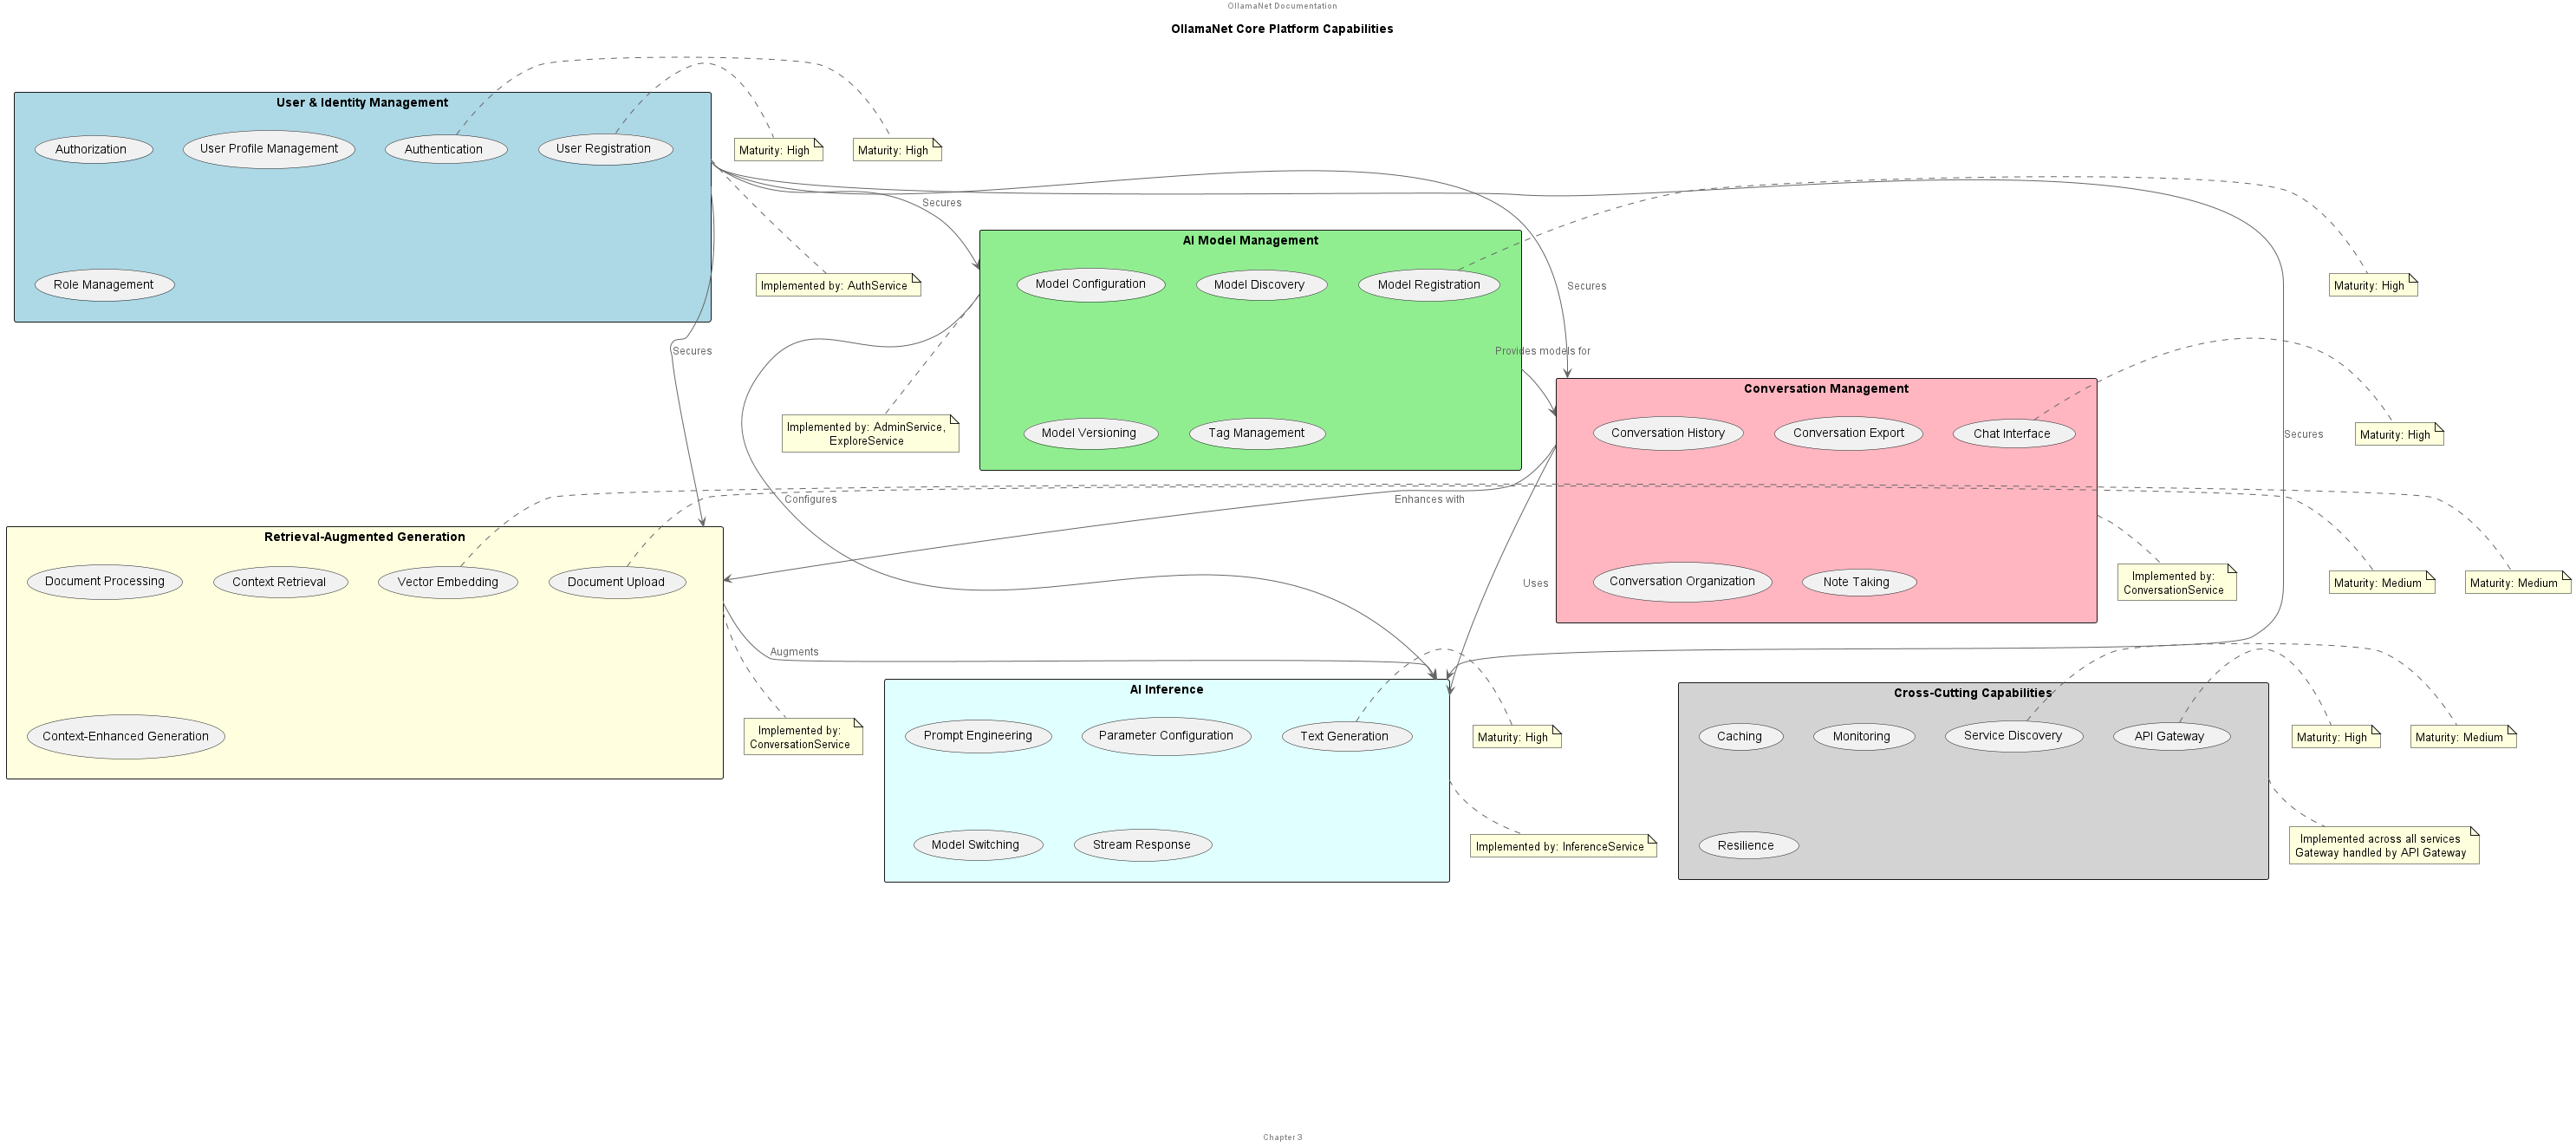
\includegraphics[width=\textwidth]{./Chapter03/figures/Core_Platform_Capabilities.png}
    \caption{Core Platform Capabilities}
    \label{fig:platform-capabilities}
\end{figure}
\clearpage

\subsection{Service-Specific Functionality Requirements}

\subsubsection*{AuthService Requirements}

\begin{enumerate}
   \item \textbf{User Account Management}
   \begin{itemize}
      \item FR-AUTH-01: The service shall allow registration of new users with email, password, and basic profile information
      \item FR-AUTH-02: The service shall validate email addresses through confirmation mechanisms
      \item FR-AUTH-03: The service shall support password reset functionality
      \item FR-AUTH-04: The service shall enforce password complexity requirements
   \end{itemize}

   \item \textbf{Authentication Mechanisms}
   \begin{itemize}
      \item FR-AUTH-05: The service shall authenticate users via username/email and password
      \item FR-AUTH-06: The service shall issue JWT tokens upon successful authentication
      \item FR-AUTH-07: The service shall support refresh tokens for maintaining sessions
      \item FR-AUTH-08: The service shall implement token revocation for security purposes
   \end{itemize}

   \item \textbf{Authorization Management}
   \begin{itemize}
      \item FR-AUTH-09: The service shall support role assignment to users
      \item FR-AUTH-10: The service shall provide APIs for role management
      \item FR-AUTH-11: The service shall enforce role-based access control
      \item FR-AUTH-12: The service shall validate tokens and claims for all protected endpoints
   \end{itemize}
\end{enumerate}

\subsubsection*{AdminService Requirements}

\begin{enumerate}
   \item \textbf{User Administration}
   \begin{itemize}
      \item FR-ADMIN-01: The service shall provide CRUD operations for user management
      \item FR-ADMIN-02: The service shall support role assignment and revocation
      \item FR-ADMIN-03: The service shall enable account status management (activation/deactivation)
      \item FR-ADMIN-04: The service shall support bulk operations for administrative efficiency
   \end{itemize}

   \item \textbf{Model Administration}
   \begin{itemize}
      \item FR-ADMIN-05: The service shall enable registration of AI models with metadata
      \item FR-ADMIN-06: The service shall provide model update and deletion capabilities
      \item FR-ADMIN-07: The service shall support model categorization through tags
      \item FR-ADMIN-08: The service shall allow model activation and deactivation
   \end{itemize}

   \item \textbf{Tag Management}
   \begin{itemize}
      \item FR-ADMIN-09: The service shall provide CRUD operations for tags
      \item FR-ADMIN-10: The service shall enable association of tags with models
      \item FR-ADMIN-11: The service shall support hierarchical tag relationships
      \item FR-ADMIN-12: The service shall provide search and filtering for tags
   \end{itemize}

   \item \textbf{Model Deployment}
   \begin{itemize}
      \item FR-ADMIN-13: The service shall connect to the Ollama API for model operations
      \item FR-ADMIN-14: The service shall support model installation with progress tracking
      \item FR-ADMIN-15: The service shall provide model information retrieval
      \item FR-ADMIN-16: The service shall enable model removal and cleanup
   \end{itemize}
\end{enumerate}

\subsubsection*{ConversationService Requirements}

\begin{enumerate}
   \item \textbf{Conversation Management}
   \begin{itemize}
      \item FR-CONV-01: The service shall provide CRUD operations for conversations
      \item FR-CONV-02: The service shall support conversation title management
      \item FR-CONV-03: The service shall enable conversation search and filtering
      \item FR-CONV-04: The service shall manage conversation archiving and deletion
   \end{itemize}

   \item \textbf{Chat Functionality}
   \begin{itemize}
      \item FR-CONV-05: The service shall enable sending messages to AI models
      \item FR-CONV-06: The service shall support streaming responses for real-time interaction
      \item FR-CONV-07: The service shall maintain conversation context for improved responses
      \item FR-CONV-08: The service shall track and report token usage
   \end{itemize}

   \item \textbf{Organization Features}
   \begin{itemize}
      \item FR-CONV-09: The service shall provide folder CRUD operations
      \item FR-CONV-10: The service shall support moving conversations between folders
      \item FR-CONV-11: The service shall enable note-taking associated with conversations
      \item FR-CONV-12: The service shall support tagging and categorization of conversations
   \end{itemize}

   \item \textbf{Document Integration}
   \begin{itemize}
      \item FR-CONV-13: The service shall enable document uploading and management
      \item FR-CONV-14: The service shall process documents for content extraction
      \item FR-CONV-15: The service shall use document content for context enhancement
      \item FR-CONV-16: The service shall support multiple document formats (PDF, TXT, DOCX)
   \end{itemize}

   \item \textbf{Feedback Collection}
   \begin{itemize}
      \item FR-CONV-17: The service shall provide mechanisms for users to rate AI responses
      \item FR-CONV-18: The service shall collect optional feedback comments
      \item FR-CONV-19: The service shall store feedback for future analysis
      \item FR-CONV-20: The service shall associate feedback with specific AI responses
   \end{itemize}
\end{enumerate}

\subsubsection*{ExploreService Requirements}

\begin{enumerate}
   \item \textbf{Model Discovery}
   \begin{itemize}
      \item FR-EXPL-01: The service shall provide a catalog of available AI models
      \item FR-EXPL-02: The service shall support browsing models by categories
      \item FR-EXPL-03: The service shall enable searching for models by keywords
      \item FR-EXPL-04: The service shall support filtering models by various attributes
   \end{itemize}

   \item \textbf{Model Information}
   \begin{itemize}
      \item FR-EXPL-05: The service shall provide detailed model metadata
      \item FR-EXPL-06: The service shall display model capabilities and specifications
      \item FR-EXPL-07: The service shall show associated tags and categories
      \item FR-EXPL-08: The service shall include model usage information when available
   \end{itemize}

   \item \textbf{Performance Optimization}
   \begin{itemize}
      \item FR-EXPL-09: The service shall implement caching for frequently accessed model data
      \item FR-EXPL-10: The service shall optimize search operations for performance
      \item FR-EXPL-11: The service shall use pagination for large result sets
      \item FR-EXPL-12: The service shall implement cache invalidation strategies
   \end{itemize}
\end{enumerate}

\subsubsection*{InferenceService Requirements}

\begin{enumerate}
   \item \textbf{Model Inference}
   \begin{itemize}
      \item FR-INF-01: The service shall provide API endpoints for AI model inference
      \item FR-INF-02: The service shall support text completion requests
      \item FR-INF-03: The service shall enable streaming responses
      \item FR-INF-04: The service shall maintain connection with the Ollama backend
   \end{itemize}

   \item \textbf{Service Discovery}
   \begin{itemize}
      \item FR-INF-05: The service shall dynamically publish its endpoint URL
      \item FR-INF-06: The service shall use RabbitMQ for service discovery messages
      \item FR-INF-07: The service shall implement secure tunneling via ngrok
      \item FR-INF-08: The service shall provide health check endpoints
   \end{itemize}

   \item \textbf{Notebook Integration}
   \begin{itemize}
      \item FR-INF-09: The service shall operate in cloud notebook environments
      \item FR-INF-10: The service shall handle environment initialization
      \item FR-INF-11: The service shall manage Ollama and ngrok processes
      \item FR-INF-12: The service shall provide interactive operation controls
   \end{itemize}
\end{enumerate}

\subsection{API Requirements}

The OllamaNet platform's APIs must adhere to the following requirements:

\begin{enumerate}
   \item \textbf{REST Principles}
   \begin{itemize}
      \item The APIs shall follow RESTful design practices
      \item The APIs shall use standard HTTP verbs appropriately (GET, POST, PUT, DELETE)
      \item The APIs shall return appropriate HTTP status codes
      \item The APIs shall implement proper resource naming conventions
   \end{itemize}

   \item \textbf{API Documentation}
   \begin{itemize}
      \item All APIs shall be documented using Swagger/OpenAPI
      \item API documentation shall include endpoint descriptions, parameters, and response formats
      \item API documentation shall be available through interactive endpoints
      \item API documentation shall include example requests and responses
   \end{itemize}

   \item \textbf{Request/Response Format}
   \begin{itemize}
      \item APIs shall accept and return data in JSON format
      \item APIs shall implement consistent request validation
      \item APIs shall provide clear error messages and codes
      \item APIs shall use pagination for large result sets
   \end{itemize}

   \item \textbf{Security Controls}
   \begin{itemize}
      \item APIs shall require authentication for protected resources
      \item APIs shall validate JWT tokens for protected endpoints
      \item APIs shall implement appropriate CORS policies
      \item APIs shall sanitize inputs to prevent injection attacks
   \end{itemize}

   \item \textbf{Versioning}
   \begin{itemize}
      \item APIs shall support versioning to maintain backward compatibility
      \item API versions shall be included in the URL path
      \item API changes shall be documented between versions
      \item Deprecated API versions shall be clearly marked
   \end{itemize}
\end{enumerate}

\subsection{Integration Requirements}

The OllamaNet platform requires the following integration capabilities:

\begin{enumerate}
   \item \textbf{Service-to-Service Communication}
   \begin{itemize}
      \item Services shall communicate via well-defined APIs
      \item Services shall handle communication errors gracefully
      \item Services shall implement circuit breakers for resilience
      \item Services shall validate data received from other services
   \end{itemize}

   \item \textbf{External System Integration}
   \begin{itemize}
      \item The platform shall integrate with Ollama for model inference
      \item The platform shall support ngrok for dynamic service exposure
      \item The platform shall implement RabbitMQ for messaging and service discovery
      \item The platform shall provide extensibility points for future integrations
   \end{itemize}

   \item \textbf{Frontend Integration}
   \begin{itemize}
      \item The platform shall provide APIs suitable for frontend consumption
      \item The platform shall implement appropriate CORS settings
      \item The platform shall support real-time features through streaming APIs
      \item The platform shall implement API rate limiting for fairness
   \end{itemize}

   \item \textbf{Data Synchronization}
   \begin{itemize}
      \item The platform shall maintain data consistency across services
      \item The platform shall implement appropriate caching strategies
      \item The platform shall handle concurrent modifications appropriately
      \item The platform shall provide mechanisms for data reconciliation
   \end{itemize}
\end{enumerate}

\subsection{Security and Access Control Requirements}

\begin{enumerate}
   \item \textbf{Authentication}
   \begin{itemize}
      \item The platform shall implement JWT-based authentication
      \item The platform shall support refresh tokens for session maintenance
      \item The platform shall enforce token expiration and validation
      \item The platform shall provide secure password management
   \end{itemize}

   \item \textbf{Authorization}
   \begin{itemize}
      \item The platform shall implement role-based access control
      \item The platform shall enforce authorization at the API Gateway level
      \item The platform shall propagate user claims to downstream services
      \item The platform shall validate permissions for protected operations
   \end{itemize}

   \item \textbf{Data Protection}
   \begin{itemize}
      \item The platform shall encrypt sensitive data at rest
      \item The platform shall use HTTPS for all communications
      \item The platform shall implement proper data isolation between users
      \item The platform shall provide secure credential storage
   \end{itemize}

   \item \textbf{Audit and Compliance}
   \begin{itemize}
      \item The platform shall maintain audit logs for security events
      \item The platform shall log authentication attempts and failures
      \item The platform shall track administrative actions
      \item The platform shall support compliance reporting
   \end{itemize}
\end{enumerate}

\subsection{Data Management Requirements}

\begin{enumerate}
   \item \textbf{Data Storage}
   \begin{itemize}
      \item The platform shall use SQL Server for relational data storage
      \item The platform shall implement proper schema design
      \item The platform shall maintain referential integrity
      \item The platform shall support data migration and evolution
   \end{itemize}

   \item \textbf{Data Access}
   \begin{itemize}
      \item The platform shall implement the repository pattern for data access
      \item The platform shall use the unit of work pattern for transaction management
      \item The platform shall provide efficient query capabilities
      \item The platform shall support pagination for large data sets
   \end{itemize}

   \item \textbf{Caching}
   \begin{itemize}
      \item The platform shall implement Redis for distributed caching
      \item The platform shall use appropriate cache expiration policies
      \item The platform shall maintain cache consistency
      \item The platform shall provide fallback mechanisms for cache failures
   \end{itemize}

   \item \textbf{Data Lifecycle}
   \begin{itemize}
      \item The platform shall support soft deletion for most entities
      \item The platform shall implement data archiving strategies
      \item The platform shall provide data export capabilities
      \item The platform shall handle data purging for compliance
   \end{itemize}
\end{enumerate}

\begin{terminology}
\begin{description}
    \item[Functional Requirement:] A requirement that specifies what the system should do
    \item[Service Capability:] A discrete function or set of functions provided by a service
\end{description}
\end{terminology}

\section{Non-Functional Requirements}

\subsection{Performance Requirements}

The OllamaNet platform must meet the following performance requirements:

\begin{enumerate}
   \item \textbf{Response Time}
   \begin{itemize}
      \item NFR-PERF-01: API endpoints shall respond within 200ms for non-computational operations
      \item NFR-PERF-02: Authentication operations shall complete within 500ms
      \item NFR-PERF-03: Database queries shall execute within 100ms for 95\% of requests
      \item NFR-PERF-04: Static resource delivery shall occur within 50ms
      \item NFR-PERF-05: AI inference first-token response shall occur within 1 second
   \end{itemize}

   \item \textbf{Throughput}
   \begin{itemize}
      \item NFR-PERF-06: The platform shall support at least 100 concurrent users per instance
      \item NFR-PERF-07: The platform shall process at least 50 API requests per second per instance
      \item NFR-PERF-08: The platform shall manage at least 25 concurrent conversation sessions per instance
      \item NFR-PERF-09: The administrative API shall handle at least 20 requests per second
      \item NFR-PERF-10: Each service shall be capable of horizontal scaling to increase throughput
   \end{itemize}

   \item \textbf{Caching Performance}
   \begin{itemize}
      \item NFR-PERF-11: Redis cache access shall complete within 10ms
      \item NFR-PERF-12: Cache hit ratio shall exceed 80\% for frequently accessed data
      \item NFR-PERF-13: JWT validation cache shall maintain a hit ratio above 90\%
      \item NFR-PERF-14: Cache invalidation shall propagate within 5 seconds
      \item NFR-PERF-15: Cache warm-up shall complete within 30 seconds of service start
   \end{itemize}

   \item \textbf{Resource Utilization}
   \begin{itemize}
      \item NFR-PERF-16: Services shall utilize less than 70\% CPU under normal load
      \item NFR-PERF-17: Memory consumption shall not exceed 2GB per service instance
      \item NFR-PERF-18: Database connections shall be pooled with a maximum of 100 connections
      \item NFR-PERF-19: Network bandwidth usage shall remain below 50Mbps under normal operations
      \item NFR-PERF-20: Disk I/O shall remain below 70\% utilization
   \end{itemize}
\end{enumerate}

\subsection{Scalability Requirements}

The OllamaNet platform must satisfy the following scalability requirements:

\begin{enumerate}
   \item \textbf{Horizontal Scaling}
   \begin{itemize}
      \item NFR-SCAL-01: All services shall support horizontal scaling through multiple instances
      \item NFR-SCAL-02: The platform shall support auto-scaling based on predefined metrics
      \item NFR-SCAL-03: Service instances shall be stateless to facilitate scaling
      \item NFR-SCAL-04: The platform shall maintain performance under load with linear resource addition
      \item NFR-SCAL-05: Node addition shall not require system restart
   \end{itemize}

   \item \textbf{Database Scalability}
   \begin{itemize}
      \item NFR-SCAL-06: The database shall support partitioning for data growth
      \item NFR-SCAL-07: The system shall support read replicas for query scaling
      \item NFR-SCAL-08: Database operations shall use appropriate indexing for scale
      \item NFR-SCAL-09: The platform shall implement database connection pooling
      \item NFR-SCAL-10: Query patterns shall be optimized for large data volumes
   \end{itemize}

   \item \textbf{Caching Scalability}
   \begin{itemize}
      \item NFR-SCAL-11: Redis cache shall support cluster mode for horizontal scaling
      \item NFR-SCAL-12: Cache size shall be configurable based on deployment environment
      \item NFR-SCAL-13: The platform shall implement multiple cache levels for scalability
      \item NFR-SCAL-14: Cache eviction policies shall optimize for memory utilization
      \item NFR-SCAL-15: The platform shall gracefully handle cache server failures
   \end{itemize}

   \item \textbf{Load Handling}
   \begin{itemize}
      \item NFR-SCAL-16: The platform shall implement rate limiting to prevent overload
      \item NFR-SCAL-17: The platform shall queue excess requests rather than reject them
      \item NFR-SCAL-18: The platform shall degrade gracefully under extreme load
      \item NFR-SCAL-19: Backend services shall implement backpressure mechanisms
      \item NFR-SCAL-20: The platform shall support traffic prioritization
   \end{itemize}
\end{enumerate}

\begin{figure}[p]
    \centering
    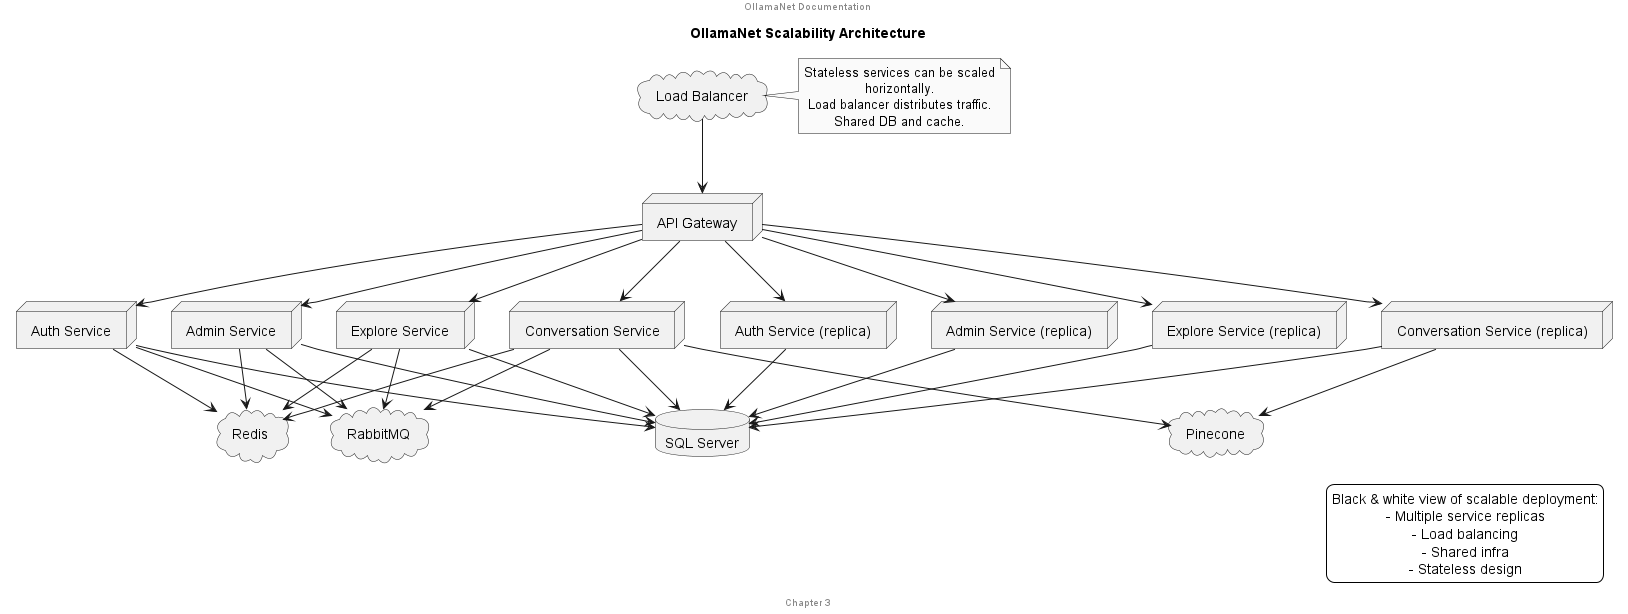
\includegraphics[width=\textwidth]{./Chapter03/figures/Scalability_Architecture.png}
    \caption{OllamaNet Scalability Architecture}
    \label{fig:scalability-architecture}
\end{figure}
\clearpage

\subsection{Security Requirements}

The OllamaNet platform must comply with the following security requirements:

\begin{enumerate}
   \item \textbf{Authentication and Authorization}
   \begin{itemize}
      \item NFR-SEC-01: User passwords shall be stored using industry-standard hashing algorithms (bcrypt)
      \item NFR-SEC-02: JWT tokens shall expire after 15 minutes of inactivity
      \item NFR-SEC-03: Refresh tokens shall expire after 30 days
      \item NFR-SEC-04: Failed login attempts shall be limited to prevent brute force attacks
      \item NFR-SEC-05: Role-based access control shall be enforced for all protected resources
   \end{itemize}

   \item \textbf{Data Protection}
   \begin{itemize}
      \item NFR-SEC-06: All communications shall use TLS 1.3 or higher
      \item NFR-SEC-07: Sensitive data shall be encrypted at rest using AES-256
      \item NFR-SEC-08: Database credentials shall be stored in secure environment variables
      \item NFR-SEC-09: Production environments shall enforce strict network isolation
      \item NFR-SEC-10: Data access shall follow the principle of least privilege
   \end{itemize}

   \item \textbf{API Security}
   \begin{itemize}
      \item NFR-SEC-11: APIs shall validate all inputs to prevent injection attacks
      \item NFR-SEC-12: CORS policies shall restrict access to approved origins
      \item NFR-SEC-13: API endpoints shall implement rate limiting
      \item NFR-SEC-14: Error responses shall not expose implementation details
      \item NFR-SEC-15: API security headers shall be implemented (HSTS, X-XSS-Protection, etc.)
   \end{itemize}

   \item \textbf{Audit and Compliance}
   \begin{itemize}
      \item NFR-SEC-16: Security-related events shall be logged with appropriate details
      \item NFR-SEC-17: Audit logs shall be immutable and tamper-evident
      \item NFR-SEC-18: The platform shall support regulatory compliance reporting
      \item NFR-SEC-19: Privileged operations shall require additional authentication
      \item NFR-SEC-20: Regular security assessments shall be supported
   \end{itemize}

   \item \textbf{Vulnerability Management}
   \begin{itemize}
      \item NFR-SEC-21: The platform shall not use components with known vulnerabilities
      \item NFR-SEC-22: The platform shall be designed to mitigate OWASP Top 10 vulnerabilities
      \item NFR-SEC-23: Security patches shall be applicable without service interruption
      \item NFR-SEC-24: Dependencies shall be regularly updated to address security issues
      \item NFR-SEC-25: Security testing shall be integrated into the development process
   \end{itemize}
\end{enumerate}

\subsection{Reliability and Availability Requirements}

The OllamaNet platform must meet the following reliability and availability requirements:

\begin{enumerate}
   \item \textbf{System Availability}
   \begin{itemize}
      \item NFR-REL-01: The platform shall maintain 99.9\% uptime (excluding planned maintenance)
      \item NFR-REL-02: Planned maintenance shall occur during off-peak hours
      \item NFR-REL-03: No single point of failure shall exist in the production environment
      \item NFR-REL-04: The system shall support rolling updates without downtime
      \item NFR-REL-05: The platform shall detect and restart failed service instances automatically
   \end{itemize}

   \item \textbf{Fault Tolerance}
   \begin{itemize}
      \item NFR-REL-06: The platform shall implement circuit breakers for external service calls
      \item NFR-REL-07: Services shall fail gracefully when dependencies are unavailable
      \item NFR-REL-08: The system shall implement retry logic with exponential backoff
      \item NFR-REL-09: The platform shall maintain data integrity during partial system failures
      \item NFR-REL-10: The system shall recover automatically from most failure scenarios
   \end{itemize}

   \item \textbf{Data Reliability}
   \begin{itemize}
      \item NFR-REL-11: The database shall use transaction isolation to prevent data corruption
      \item NFR-REL-12: The platform shall implement data backups with point-in-time recovery
      \item NFR-REL-13: Data integrity constraints shall be enforced at the database level
      \item NFR-REL-14: The system shall detect and log data inconsistencies
      \item NFR-REL-15: Critical data changes shall be audited with before/after values
   \end{itemize}

   \item \textbf{Disaster Recovery}
   \begin{itemize}
      \item NFR-REL-16: The platform shall support database failover to standby replicas
      \item NFR-REL-17: Recovery Point Objective (RPO) shall be less than 5 minutes
      \item NFR-REL-18: Recovery Time Objective (RTO) shall be less than 30 minutes
      \item NFR-REL-19: Disaster recovery procedures shall be documented and tested
      \item NFR-REL-20: The system shall support geographic redundancy for critical components
   \end{itemize}
\end{enumerate}

\subsection{Maintainability Requirements}

The OllamaNet platform must adhere to the following maintainability requirements:

\begin{enumerate}
   \item \textbf{Code Quality}
   \begin{itemize}
      \item NFR-MAIN-01: Code shall follow language-specific style guidelines
      \item NFR-MAIN-02: Code complexity metrics shall remain below specified thresholds
      \item NFR-MAIN-03: Test coverage shall exceed 80\% for critical components
      \item NFR-MAIN-04: Static code analysis shall be part of the build process
      \item NFR-MAIN-05: Code shall be properly commented and documented
   \end{itemize}

   \item \textbf{Deployment}
   \begin{itemize}
      \item NFR-MAIN-06: The platform shall support containerized deployment
      \item NFR-MAIN-07: Configuration shall be externalized from code
      \item NFR-MAIN-08: The system shall support environment-specific configuration
      \item NFR-MAIN-09: Deployment shall be automated via CI/CD pipelines
      \item NFR-MAIN-10: Deployments shall be reversible through rollback mechanisms
   \end{itemize}

   \item \textbf{Monitoring and Diagnostics}
   \begin{itemize}
      \item NFR-MAIN-11: Services shall expose health check endpoints
      \item NFR-MAIN-12: The system shall generate appropriate logs for troubleshooting
      \item NFR-MAIN-13: Performance metrics shall be collected and available for analysis
      \item NFR-MAIN-14: Error conditions shall trigger appropriate alerts
      \item NFR-MAIN-15: The platform shall support distributed tracing
   \end{itemize}

   \item \textbf{Extensibility}
   \begin{itemize}
      \item NFR-MAIN-16: The system architecture shall support adding new services
      \item NFR-MAIN-17: APIs shall be versioned to support evolution
      \item NFR-MAIN-18: The database schema shall support extension without redesign
      \item NFR-MAIN-19: User interface components shall be modular and reusable
      \item NFR-MAIN-20: The system shall support plugin architectures where appropriate
   \end{itemize}
\end{enumerate}

\subsection{Compatibility and Interoperability Requirements}

The OllamaNet platform must satisfy the following compatibility and interoperability requirements:

\begin{enumerate}
   \item \textbf{Client Compatibility}
   \begin{itemize}
      \item NFR-COMP-01: Frontend applications shall work on modern browsers (Chrome, Firefox, Safari, Edge)
      \item NFR-COMP-02: The system shall support responsive design for mobile and desktop access
      \item NFR-COMP-03: APIs shall be accessible from common programming languages
      \item NFR-COMP-04: The platform shall support common authentication mechanisms (JWT, OAuth)
      \item NFR-COMP-05: Public interfaces shall follow industry standards for maximum compatibility
   \end{itemize}

   \item \textbf{Integration Compatibility}
   \begin{itemize}
      \item NFR-COMP-06: The platform shall use standard protocols for integration (REST, AMQP)
      \item NFR-COMP-07: Data exchange shall use standardized formats (JSON, XML)
      \item NFR-COMP-08: APIs shall provide Swagger/OpenAPI documentation
      \item NFR-COMP-09: The platform shall support standard database connection mechanisms
      \item NFR-COMP-10: Integration points shall be well documented for third-party developers
   \end{itemize}

   \item \textbf{Environment Compatibility}
   \begin{itemize}
      \item NFR-COMP-11: The platform shall operate in common cloud environments (AWS, Azure, GCP)
      \item NFR-COMP-12:
     \end{itemize}
  
   \end{enumerate}




